\documentclass[11pt,a4j]{jsarticle}

\usepackage{float,array,booktabs,here}
\usepackage{amsmath}
\usepackage[dvipdfmx]{graphicx}
\usepackage[top=20truemm,bottom=25truemm,left=20truemm,right=20truemm]{geometry}
\usepackage{url}
\usepackage{listings, jlisting}

\lstset{language=c,
  frame=single,
  stepnumber=1,
  numbersep=2pt,
  tabsize=2,
  basicstyle=\verysmall\ttfamily,
  stringstyle=\small\texttt,
  commentstyle=\slshape,
  captionpos=b,
  columns=[l]{fullflexible}
}

\makeatletter
\newcommand{\figcaption}[1]{\def\@captype{figure}\caption{#1}}
\newcommand{\tblcaption}[1]{\def\@captype{table}\caption{#1}}
\makeatother

\newcommand{\Maru}[1]{\ooalign{
\ifnum#1<10 \hfil\resizebox{.9\width}{.85\height}{#1}\hfil
\else
\hfil\resizebox{.6\width}{.8\height}{#1}\hfil
\fi
\crcr
\raise.1ex\hbox{$\bigcirc$}}}


\begin{document}

\input{title}

\section{サンプリング対象}

``booking.com''に掲載されている、人気度順にソートした30位までの東京都のホテルの2人での宿泊代金。

また日程をクリスマス(12/24(土))と(10/29(土))の2日程にすることで比較も行ってみる。


\section{目的・対象を選んだ理由}
クリスマスにホテルの宿泊代金は上昇するのか。

自分がクリスマスに宿泊をしたかったため、ホテルを探しているうちに、クリスマスだからこその価格の上昇が
あるのかと興味を持ち、また周りのホテルを探す人の求めているものについても考察してみたかったため。

\section{データ表}

\begin{table}[H]
  \caption{ホテルの宿泊代金}
  \label{tab:hotel1}
  \small
  \begin{center}
      \begin{tabular}{c|cc}
        \hline
        \toprule
        順位 & 1027の宿泊代金 & 12/24の宿泊代金 \\
        \midrule
        1	&	12700	&	10400	\\
        2	&	18500	&	12100	\\
        3	&	22800	&	8600	\\
        4	&	14950	&	11500	\\
        5	&	16100	&	19500	\\
        6	&	22000	&	14400	\\
        7	&	16500	&	13000	\\
        8	&	18150	&	18000	\\
        9	&	36000	&	12000	\\
        10	&	24401	&	10400	\\
        11	&	24000	&	11820	\\
        12	&	16000	&	10200	\\
        13	&	22000	&	27500	\\
        14	&	31500	&	12000	\\
        15	&	17000	&	13750	\\
        16	&	18000	&	13000	\\
        17	&	14000	&	27000	\\
        18	&	25000	&	17000	\\
        19	&	14200	&	10400	\\
        20	&	24800	&	13000	\\
        21	&	18000	&	11200	\\
        22	&	40000	&	11000	\\
        23	&	28000	&	20000	\\
        24	&	21000	&	15000	\\
        25	&	19000	&	10726	\\
        26	&	42100	&	17500	\\
        27	&	35640	&	15500	\\
        28	&	36000	&	13200	\\
        29	&	21500	&	31200	\\
        30	&	28900	&	33000	\\
        \hline
      \end{tabular}
  \end{center}
\end{table}

\section{度数分布表}

\begin{table}[H]
  \caption{10/27の宿泊代金の度数分布表}
  \label{tab:dosuu1}
  \small
  \begin{center}
      \begin{tabular}{c|c|c|c}
        \hline
        \toprule
        価格(万円) & 階級値 & 度数 & 相対度数(\verb|%|) \\
        \midrule
        〜1	&		&	1	&	3.3	\\
        1〜1.3	&	1.15	&	15	&	50.0	\\
        1.3〜1.6	&	1.45	&	5	&	16.7	\\
        1.6〜1.9	&	1.75	&	3	&	10.0	\\
        1.9〜2.2	&	2.05	&	2	&	6.7	\\
        2.2〜2.5	&	2.35	&	0	&	0.0	\\
        2.5〜2.8	&	2.65	&	2	&	6.7	\\
        2.8〜3.1	&	2.95	&	0	&	0.0	\\
        3.1〜3.4	&	3.25	&	2	&	6.7	\\
        3.4〜3.7	&	3.55	&	0	&	0.0	\\
        3.7〜	&		&	0	&	0.0	\\
        \hline
      \end{tabular}
  \end{center}
\end{table}

\begin{table}[H]
  \caption{12/24の宿泊代金の度数分布表}
  \label{tab:dosuu2}
  \small
  \begin{center}
      \begin{tabular}{c|c|c|c}
        \hline
        \toprule
        価格(万円) & 階級値 & 度数 & 相対度数(\verb|%|) \\
        \midrule
        〜1	&		&	0	&	0.0	\\
        1〜1.3	&	1.15	&	1	&	3.3	\\
        1.3〜1.6	&	1.45	&	4	&	13.3	\\
        1.6〜1.9	&	1.75	&	8	&	26.7	\\
        1.9〜2.2	&	2.05	&	5	&	16.7	\\
        2.2〜2.5	&	2.35	&	5	&	16.7	\\
        2.5〜2.8	&	2.65	&	1	&	3.3	\\
        2.8〜3.1	&	2.95	&	1	&	3.3	\\
        3.1〜3.4	&	3.25	&	1	&	3.3	\\
        3.4〜3.7	&	3.55	&	3	&	10.0	\\
        3.7〜	&		&	1	&	3.3	\\
        \hline
      \end{tabular}
  \end{center}
\end{table}

\begin{figure}[H]
  \centering
  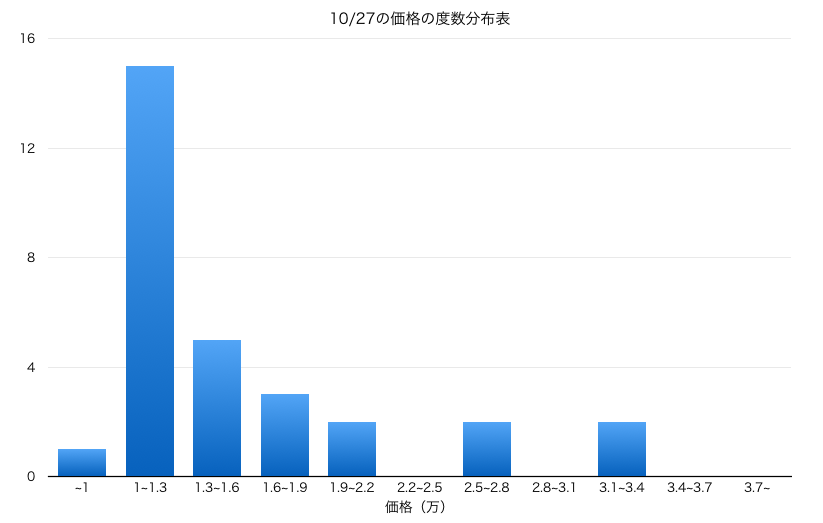
\includegraphics[height=80mm,bb=0 0 823 523]{img/1027.png}
  \figcaption{1027の宿泊代金}
  \label{fig:1027}
\end{figure}

\begin{figure}[H]
  \centering
  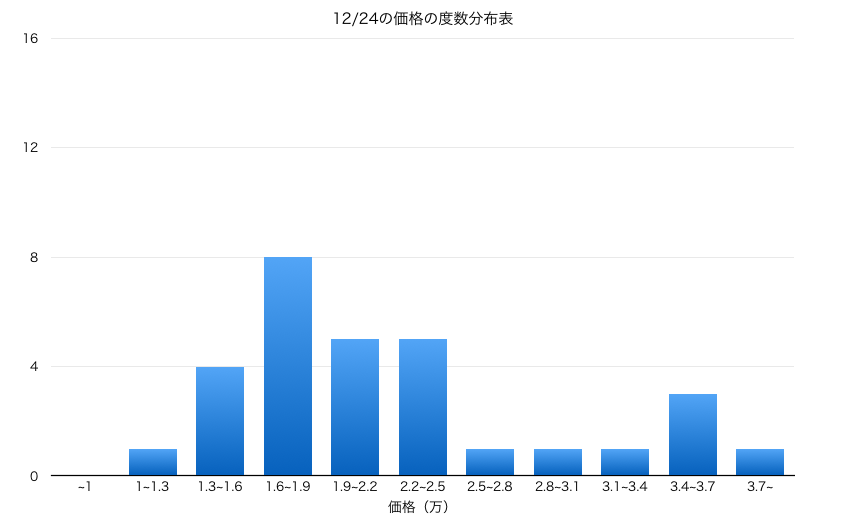
\includegraphics[height=80mm,bb=0 0 841 528]{img/1224.png}
  \figcaption{1027の宿泊代金}
  \label{fig:1027}
\end{figure}

\section{代表値}

\subsection{1027の宿泊代金について}

\begin{itemize}
  \item 相加平均: 15463円
  \item 相乗平均: 14475円
  \item 分散: 39570844
  \item 標準偏差: 6290
\end{itemize}

\subsection{1224の宿泊代金について}

\begin{itemize}
  \item 相加平均: 23291円
  \item 相乗平均: 22056円
  \item 分散: 63785019
  \item 標準偏差: 7987
\end{itemize}

\section{正規分布との比較}

1027の宿泊代は正規分布に近しい形をしている。
原因としては、booking.comのシステム上、現時点で売れ残っている部屋がランキング形式で並んでいるので
ホテル側が売り切りを目的として割引を行っている可能性があるからである。

1224の宿泊代は正規分布には沿っていない。
原因としては、クリスマスイブということもあってか多くのお金を出してもいいと思う人が多いからであると判断できる。
形として、普段の価格より少し高いところに一番の山が動いて、高額なところにもう一つの山が生まれるというところから
上記の心理については伺うことができるのではないだろうか。

\section{95%の信頼区間での平均の推定}

t分布を使って信頼区間を算出する。自由度は 30 - 1 = 29である。
df = 29として p = 0.025のt値を求めると2.056である。

\subsection{1027の宿泊代金について}

\begin{align*}
  15463 - 2.056 \frac{6290}{\sqrt{29}} \leq &\mu \leq 15463 + 2.056 \frac{6290}{\sqrt{29}} \\
  13062 \leq &\mu \leq 17864
\end{align*}

よって、13062円〜17864円である。

\subsection{1224の宿泊代金について}

\begin{align*}
  23291 - 2.056 \frac{7987}{\sqrt{29}} \leq &\mu \leq 23291 + 2.056 \frac{7987}{\sqrt{29}} \\
  20242 \leq &\mu \leq 26340
\end{align*}

よって、20242円〜26340円である。

\section{結論}

もっと大きなDBがあれば多くの標本で調べることができるため、そうするともっと面白そうである。

曜日を揃えて比較したのは良かったが、直前の割引をもう少し考慮して
1224と1217で比較するのがベストであったかもしれないと、検討後に気づいた。

ランキングで並べると、クリスマスに高級ホテルを求めるであろうという予想に従った結果となったのは
興味深かった。


\end{document}
